\section{(E,+) group}

\subsection{Non associative binary operation}
\begin{frame}[t]
    \frametitle{Non associative binary operation}
    
    \begin{figure}[h]
        \centering
        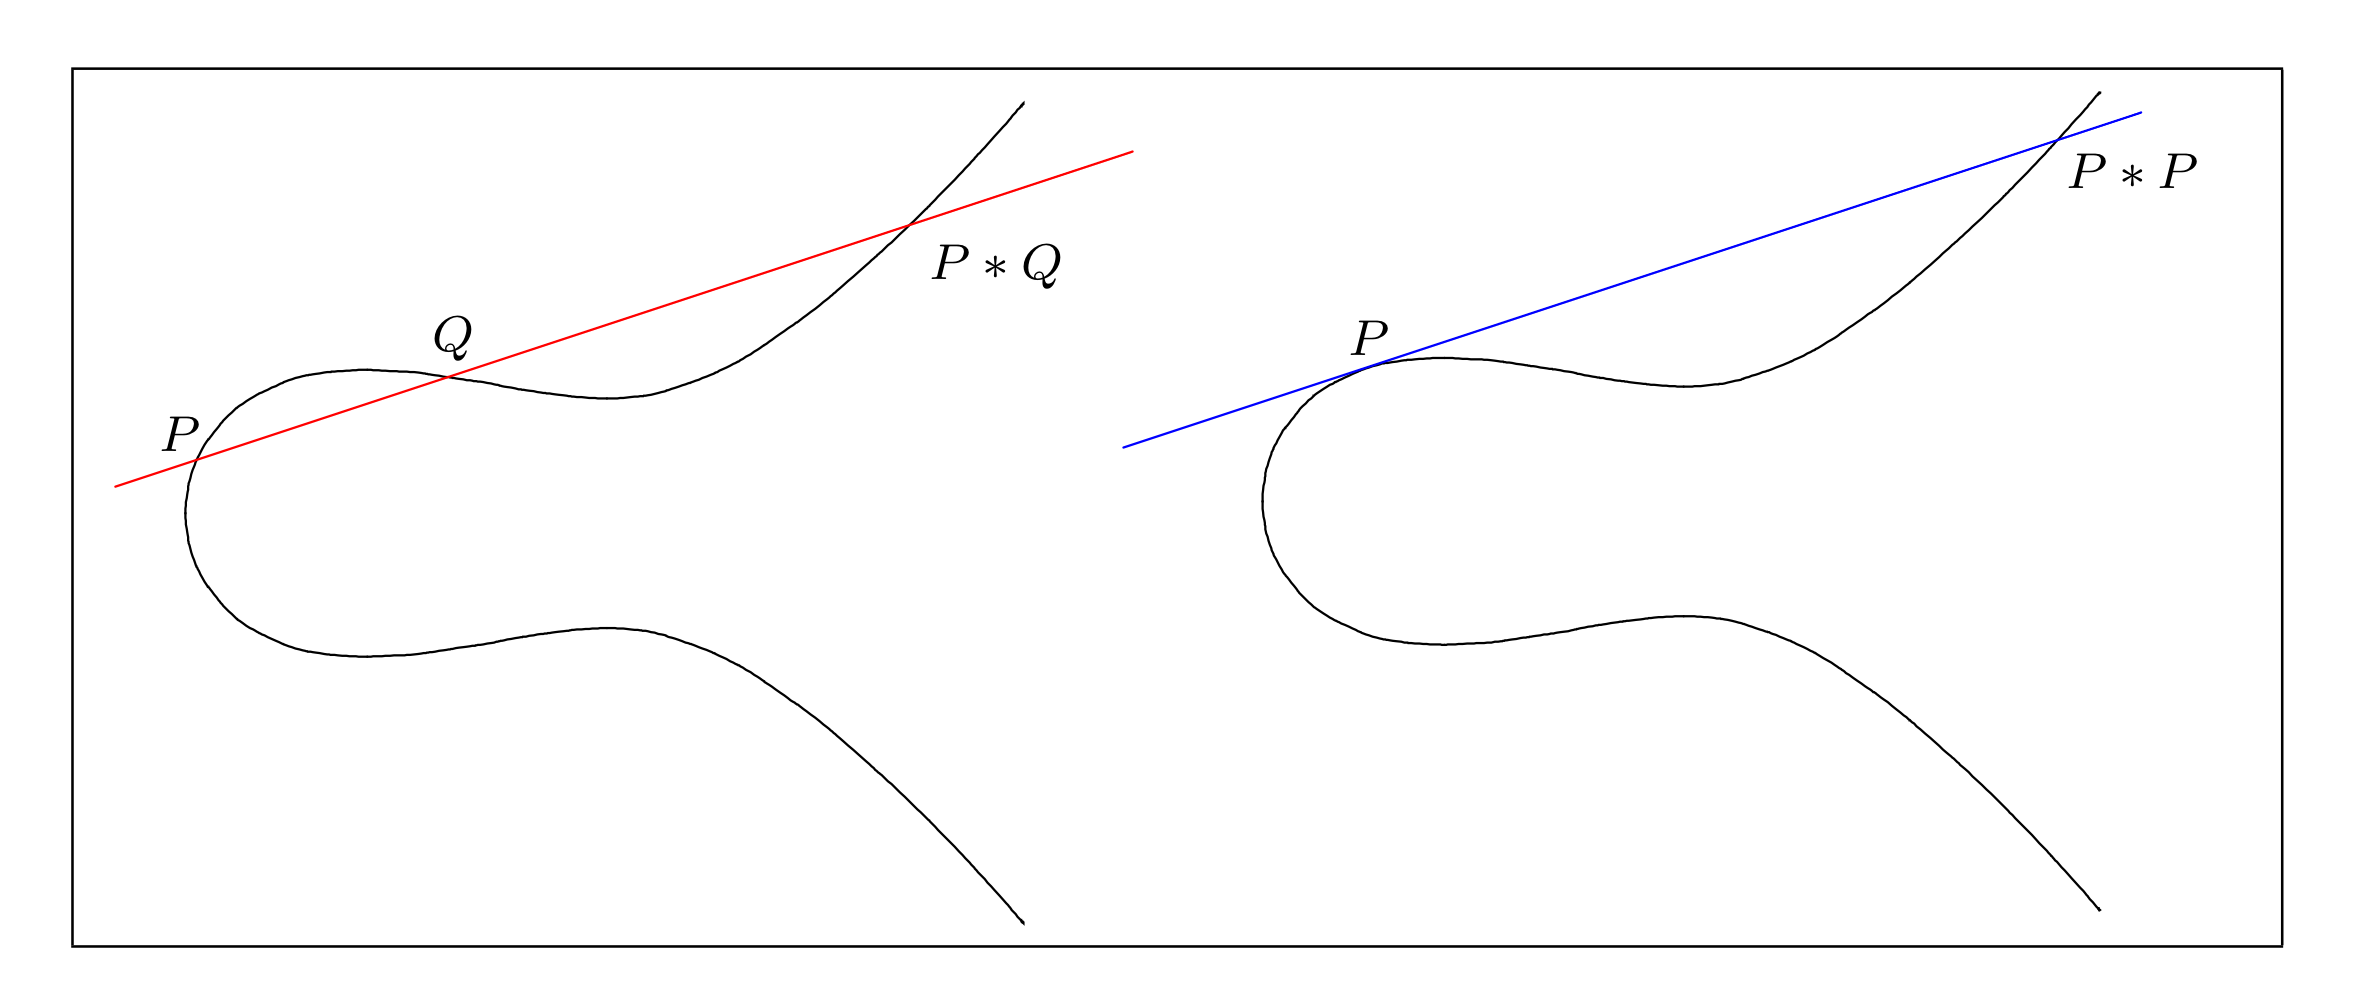
\includegraphics[width=0.8\textwidth]{cordesTangentes}
        \caption{binary operation of chord and tangent of the curve}
        \label{fig:cordesTangentes}
    \end{figure}
\end{frame}

\subsection{(E,+) abelian binary operation}
\begin{frame}[t]
    \frametitle{Abelian group}
    \begin{figure}[h]
        \centering
        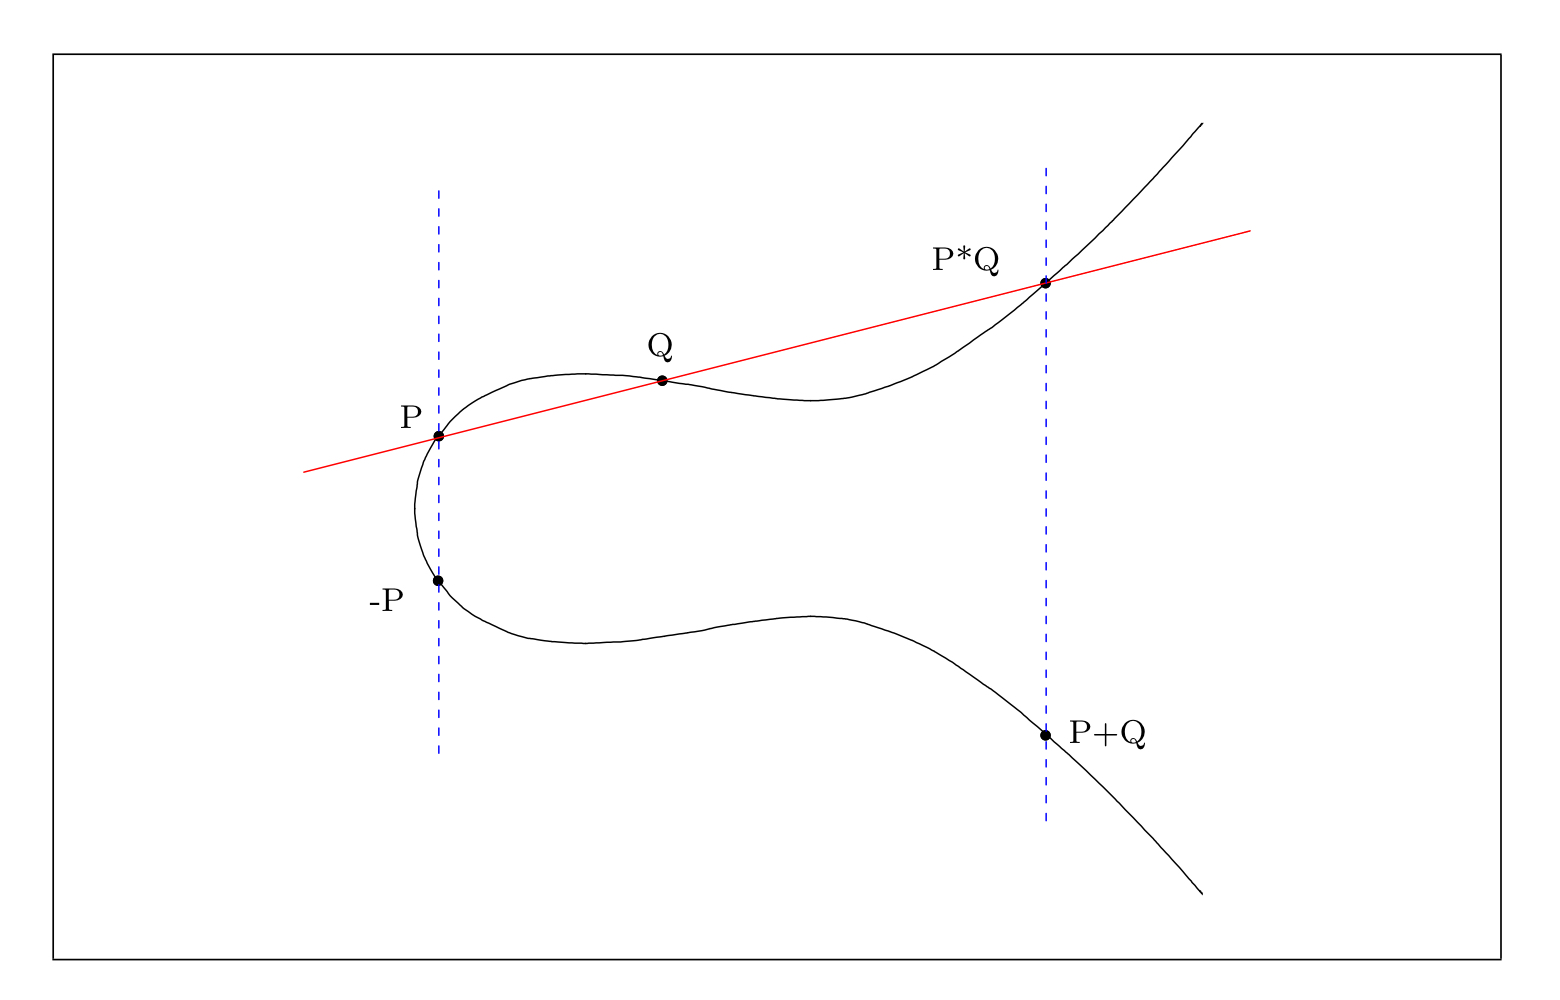
\includegraphics[width=0.7\textwidth]{loiGroupe}
        \caption{Geometric representation of the addition of rational points}
        \label{fig:loiGroupe}
    \end{figure}
\end{frame}
